\section{Analysis}
\label{sec:analysis}

\begin{figure}[t]
\centering
\vspace{-0.5cm}
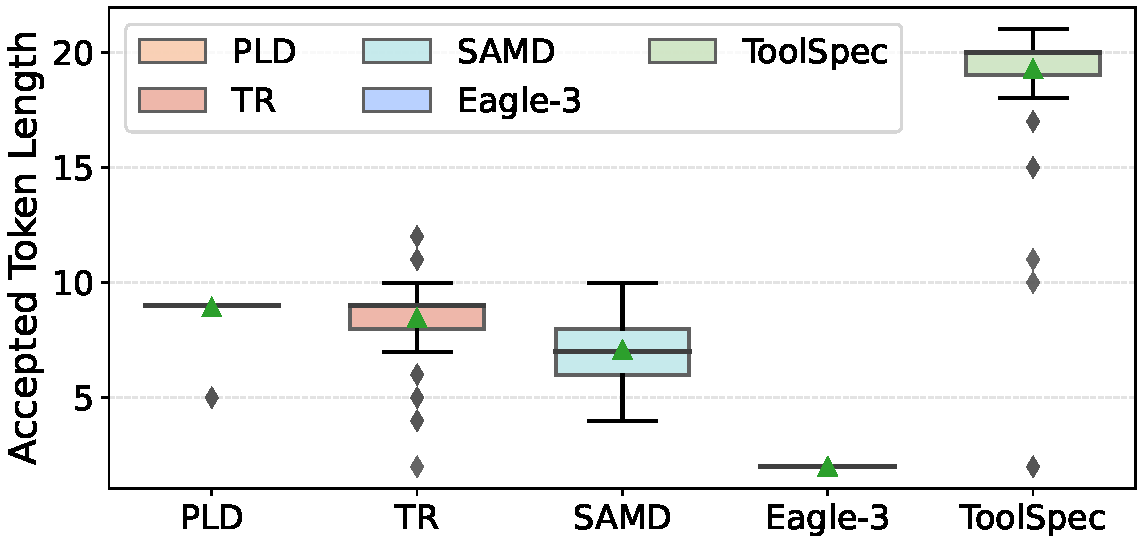
\includegraphics[width=0.95\columnwidth]{fig/first2step.pdf}
\caption{Distribution of accepted token lengths in the first two decoding steps using LLaMA-3.1-8B-Instruct on API-Bank. Green triangles represent mean values, and black diamonds denote outliers.}
\label{fig:first2token}
\end{figure}

This section presents a comprehensive analysis of \method. Specifically, we evaluate its effectiveness (\S\ref{sec:effectiveness}), examine the impact of adherence to the tool-calling format (\S\ref{sec:adherence_impact}), and analyze the time allocation across different modules (\S\ref{sec:profile}).

\subsection{Effectiveness of \method}
\label{sec:effectiveness}

\begin{figure}[t]
\centering
\vspace{-0.5cm}
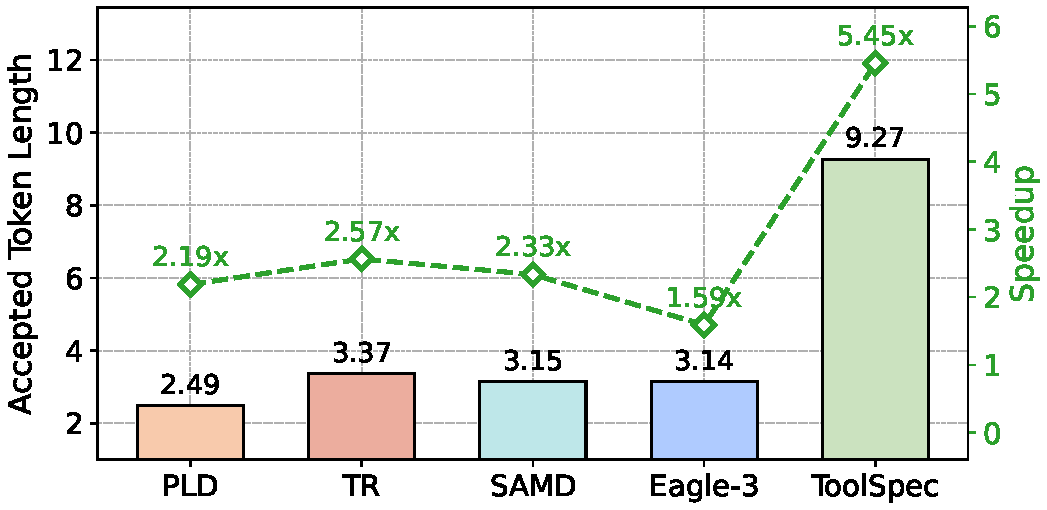
\includegraphics[width=0.95\columnwidth]{fig/repeat_call.pdf}
\caption{Mean number of accepted tokens (\#MAT) and speedups for repeated tool calls. Results are obtained using LLaMA-3.1-8B-Instruct on API-Bank.}
\label{fig:repeat_call}
\end{figure}

\paragraph{Statistical Analysis}
We first conduct a statistical evaluation to assess the effectiveness of the proposed modules, including: \textbf{1) Schema-aware Drafting.} Figure~\ref{fig:first2token} reports accepted token lengths in the first two decoding steps, corresponding to the tool-name state $q_t$ and the first parameter-name state $q_p$ in \method. As shown, schema-aware drafting enables \method to generate an average of $19.3$ tokens across these steps. In contrast, prior approaches such as TR produce an average of $8.5$ tokens, while Eagle-3 yields only $2$ tokens on average, equivalent to standard autoregressive decoding. These results demonstrate the clear advantage of schema-aware drafting for tool-calling generation. \textbf{2) Retrieval-augmented Speculation.} Figure~\ref{fig:repeat_call} presents \#MAT for repeated tool calls. The results indicate that \method consistently outperforms prior methods, achieving an average of $9.3$ accepted tokens per decoding step and approximately $5.5\times$ speedup. This improvement highlights the effectiveness of the proposed retrieval strategy in handling repetitive tool invocations.

\begin{figure}[t]
\centering
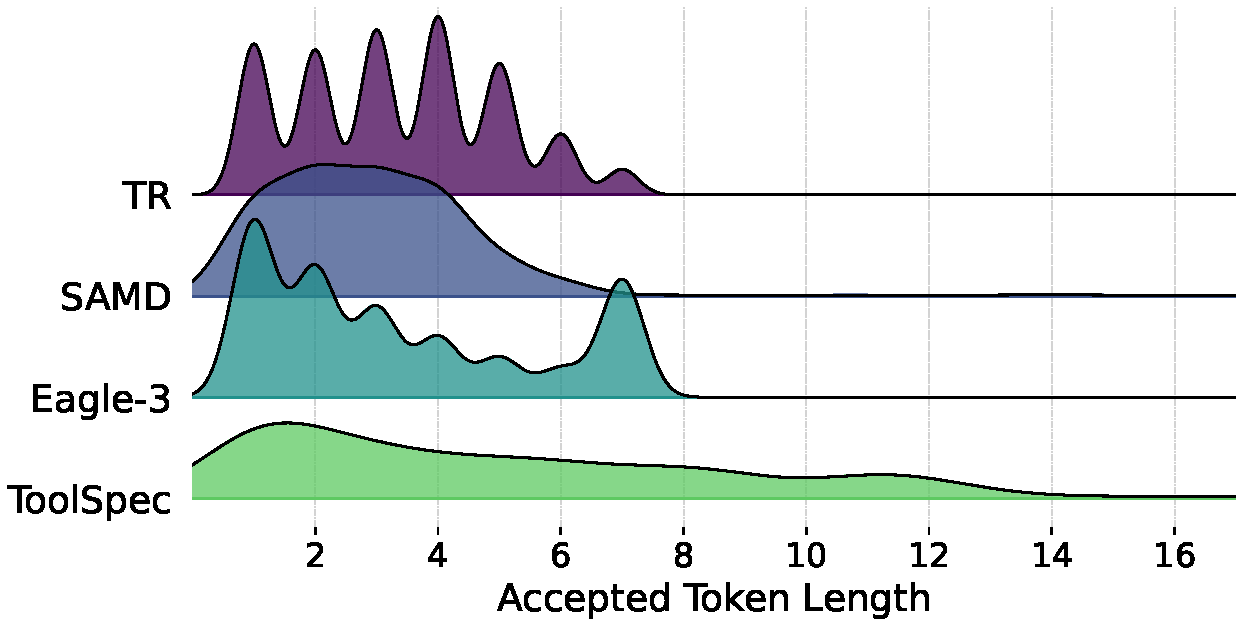
\includegraphics[width=0.95\columnwidth]{fig/accept_length_ridge.pdf}
\caption{Distribution of accepted token lengths using LLaMA-3.1-8B-Instruct on API-Bank. Values exceeding 17 are truncated for clearer visualization.}
\vspace{-0.3cm}
\label{fig:ridge}
\end{figure}

\paragraph{Acceptance Distribution}
Figure~\ref{fig:ridge} presents the distribution of accepted token lengths for \method in comparison with prior methods. While existing approaches typically yield accepted token lengths of fewer than $8$ tokens, \method shifts the distribution toward longer accepted lengths, with $22\%$ of decoding steps exceeding $8$ tokens. Furthermore, \method exhibits a pronounced long-tail distribution: nearly $4\%$ of decoding steps attain accepted token lengths between $17$ and $33$. This long-tail behavior stems from retrieval-augmented speculation, which reuses historical tool-call trajectories to produce longer and more accurate drafts. These consistently higher accepted token lengths contribute to the overall speedup achieved by \method.

\begin{table}[t]
\centering
\vspace{-0.5cm}
\small
\begin{tabular}{@{}l|ccc@{}}
\toprule
\bf Methods &\#MAT &Tokens/s & Speedup \\\midrule
Vanilla & 1.00 & 28.21 & 1.00$\times$ \\ \midrule
\method & \bf{5.80} & \bf{125.59} & \bf{4.45$\times$}  \\
\quad \textit{w/o SAD} & 5.58 & 118.99 & 4.22$\times$ \\
\quad \textit{w/o RAS} & 4.29 & 94.53 & 3.35$\times$ \\
\quad \textit{w/o both} & 3.62 & 76.00 & 2.69$\times$  \\
\bottomrule
\end{tabular}
\caption{Ablation study of \method modules. ``\textit{SAD}'' and ``\textit{RAS}'' denote schema-aware drafting and retrieval-augmented speculation, respectively. Results are obtained with LLaMA-3.1-8B-Instruct on API-Bank.}
\label{tab:ablation}
\end{table}

\paragraph{Ablation Study}
Table~\ref{tab:ablation} illustrates an ablation study of \method and its proposed components. The results indicate that both schema-aware drafting and retrieval-augmented speculation are critical to the efficiency of \method. When these components are removed, similar to PLD, \method relies on suffix matching within the input context, resulting in slightly higher speedup than TR.

\begin{figure}[t]
\centering
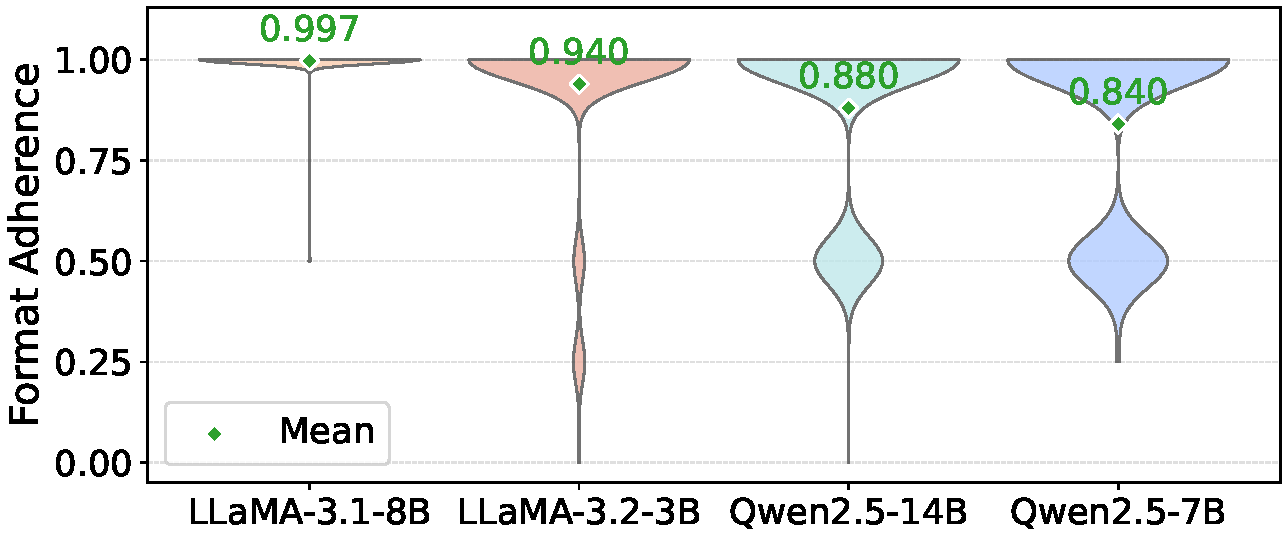
\includegraphics[width=0.95\columnwidth]{fig/violin.pdf}
\caption{Format adherence of different models in tool-calling generation. Results are obtained on API-Bank.}
\label{fig:adherence}
\end{figure}

\subsection{Impact of Format Adherence}
\label{sec:adherence_impact}
Beyond the analysis in Section~\ref{sec:pattern_analysis}, we further evaluate how strictly tool-use LLMs follow the required schema during tool-calling generation. We define strict format adherence using two criteria: 1) the outputs must be correctly parsed as valid JSON; and 2) any extraneous natural language, Markdown fences, XML-like tags, or malformed JSON structures are treated as violations. The results reveal a strong positive correlation between format adherence and the speedup achieved by \method, with a Pearson correlation coefficient of approximately $0.90$. Notably, LLaMA-3.1-8B-Instruct achieves the highest adherence score of $0.997$, corresponding to a $4.45\times$ speedup on API-Bank.

\begin{figure}[t]
\centering
\vspace{-0.5cm}
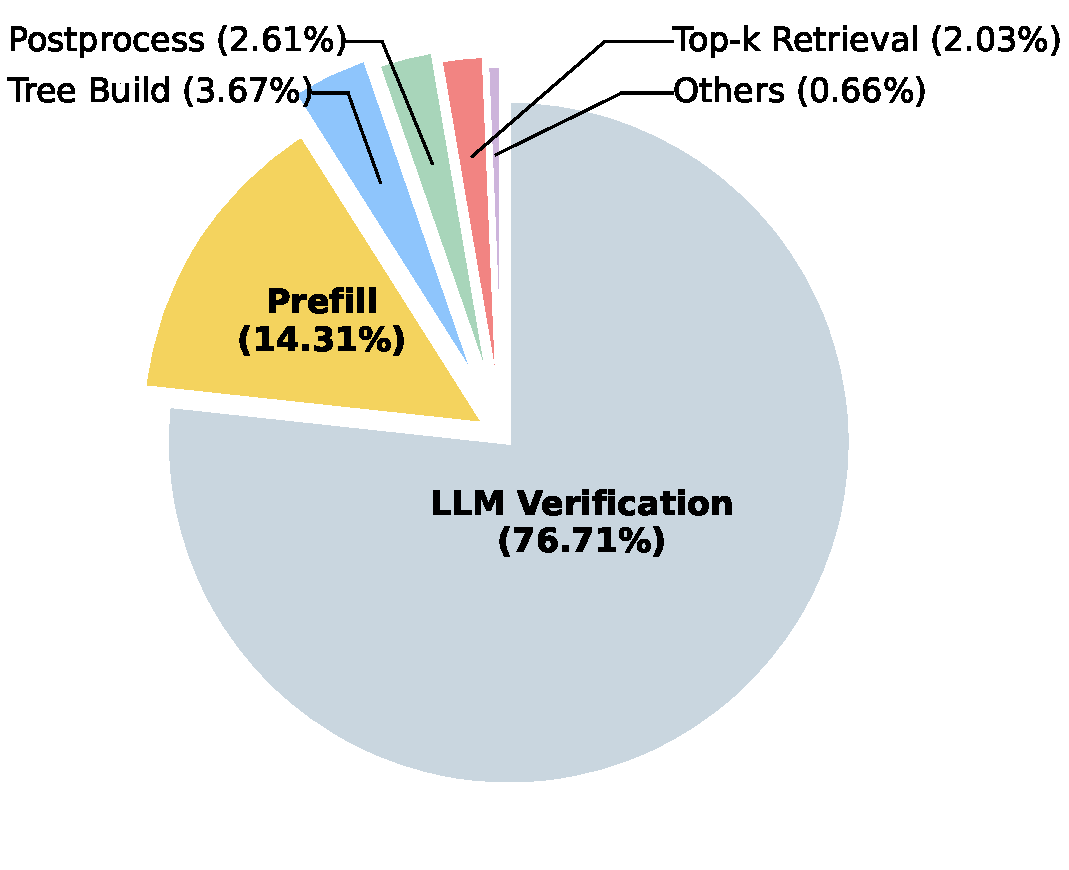
\includegraphics[width=0.85\columnwidth]{fig/profile.pdf}
\caption{Time allocation for each operation when LLMs respond to a query. Results are obtained using LLaMA-3.1-8B-Instruct on API-Bank.}
\label{fig:profile}
\end{figure}

\subsection{Time Allocation}
\label{sec:profile}

Figure~\ref{fig:profile} presents the time allocation across the primary latency-intensive components of \method. As shown, the decoding stage of the target model dominates overall latency, accounting for $91.0\%$ of the total runtime. In contrast, the additional operations introduced by \method, including top-$k$ retrieval and draft tree construction, incur only modest overhead, contributing just $5.7\%$ of the total latency. Despite this minimal overhead, \method achieves an approximately $4\times$ speedup in tool-calling generation, demonstrating its effectiveness in reducing end-to-end latency.

